\documentclass[a4paper, 12pt]{article}
\usepackage[utf8]{inputenc}
\usepackage[spanish]{babel}
\usepackage{fancyhdr}
\usepackage{gantt}
\usepackage{graphicx}
\pagestyle{fancy}

\headheight = 15pt
\title{Informe - pychat}
\author{Gustav Svensk}
\begin{document}
\lhead{Gustav Svensk}
\rhead{pychat}
\cfoot{\thepage}
\renewcommand{\headrulewidth}{0.4pt}
% \renewcommand{\footrulewidth}{0.4pt}


\maketitle
\thispagestyle{empty}
\begin{center}
        {\large Versión 0.1}
\end{center}
\newpage

\setcounter{page}{1}
\tableofcontents
\listoftables
\listoffigures
\newpage

\section{Resumen}
\subsection{Equipo}
Sólo hay un integrante del equipo, Gustav Svensk, que tendrá todos los roles del
equipo.
\subsection{Descripción}
El proyecto va a consistir en un programa chat de tipo P2P. Sólo se
podrá chatear entre dos personas (no puede estar 3 personas en el mismo
chat).

El programa tendrá una interfaz básica basado en parte en la linea de comandos.

El programa será escrito en Python.
\subsection{Requerimientos}
En esta sección se escribe los requerimientos del programa.
\subsubsection{HW}
\begin{itemize}
        \item Computadora conectado al Internet capaz a correr python
        \item Puede ser que se necesitará acceso a un router para cambiar el
                reenvío de puertos.
\end{itemize}
\subsubsection{SW}
\begin{itemize}
        \item Python 3.x
        \item PyQt4
        \item Qt4
        \item (PyTest para verificación de funcionamiento)
\end{itemize}
\subsection{Tablas GANTT}
\subsubsection{Tabla inicial}
\begin{gantt}[xunitlength=5mm]{8}{15}
\begin{ganttitle}
        \numtitle{2}{2}{30}{1}
\end{ganttitle}
\ganttbar{Recibir mensaje}{0}{3}
\ganttbarcon{Enviar mensaje}{3}{2}
\ganttbarcon{Parse mensaje}{5}{1}
\ganttbar{GUI}{6}{2}
\ganttbar{Consola}{8}{2}
\ganttbar{Concurrencia}{10}{3}
\ganttbarcon{Verificación}{13}{2}
\ganttcon{5}{2}{13}{7}
\end{gantt}

\subsubsection{Tabla final}
\begin{gantt}[xunitlength=5mm]{8}{19}
\begin{ganttitle}
        \numtitle{2}{2}{38}{1}
\end{ganttitle}
\ganttbar{Recibir mensaje}{0}{4}
\ganttbarcon{Enviar mensaje}{4}{2}
\ganttbarcon{Parse mensaje}{6}{1}
\ganttbar{GUI}{7}{2}
\ganttbar{Consola}{9}{2}
\ganttbar{Concurrencia}{11}{4}
\ganttbarcon{Verificación}{15}{4}
\ganttcon{5}{2}{15}{7}
\end{gantt}

Como se puede ver en las tablas Gantt el proyecto tomó más tiempo que planeado.
Las cosas que tomaron más tiempo era hacer el socket de bienvenido en su propia
hebra y trabajar con la concurrencia. También había varios errores pequeños en
el fin del proyecto que hacían que la verificación tomaba más tiempo.

\subsection{Resultados}
El programa funciona ahora pero para ser más fácil a usar se debería cambiar la
interfaz para que sea más intuitiva. He aprendido que concurrencia, interfaces
gráficas y comunicación entre procesos/hebras puede causar muchos problemas y a
veces se necesita cambiar su estructura inicial para habilitar restricciones de
otros programas. En este caso había problemas a correr la interfaz gráfica en una
hebra que no era la hebra principal. Por eso la interfaz corre en su propio
proceso ahora y se necesita comunicación entre procesos en vez que comunicación
entre hebras que es más fácil.

\section{Arquitectura}
La arquitectura del programa es P2P, usa sockets TCP y es escrito en Python3.
En figura~\ref{fig:arch} se puede ver un diagrama de la arquitectura del
programa.
\begin{figure}[hb]
        \centering
        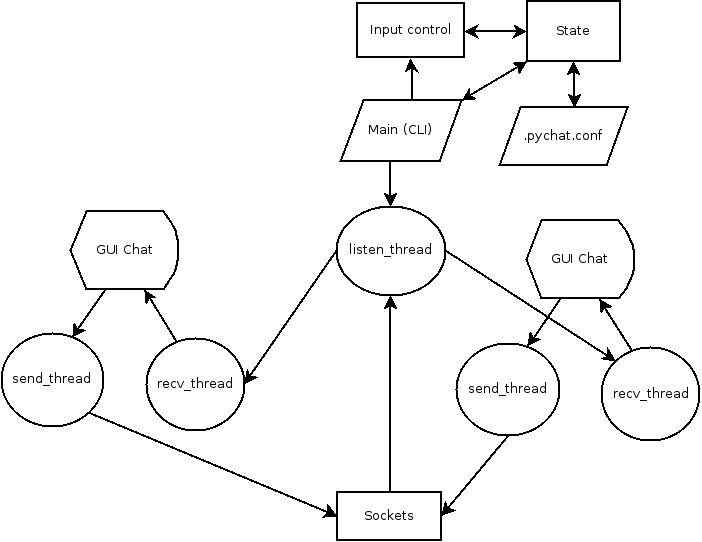
\includegraphics[width=\textwidth]{../imagenes/architecture.png}
        \caption{Diagrama de Arquitectura}
        \label{fig:arch}
\end{figure}
\begin{itemize}
        \item \texttt{Main(CLI)} - La hebra principal que inicia y maneja los otros
                objetos
        \item \texttt{Input Control} - El objeto que maneja las entradas de la linea de
                commandos
        \item \texttt{State} - El objeto que contiene el estado del programa, por
                ejemplo que chats son abiertos, guarda los amigos y los objetos
                para comunicación entre procesos
        \item \texttt{.pychat.conf} - Archivo que guarda los amigos

        \item \texttt{listen\_thread} - La hebrea que contiene el socket del ``servidor'',
                todos los mensajes recibidos van por este socket que en su torno
                busca a que chat van y los envía por allí
        \item \texttt{GUI Chat} - La interfaz gráfica de cada chat abierto
        \item \texttt{send\_thread} - La hebra que envía los mensajes del chat
        \item \texttt{recv\_thread} - La hebra que recibe mensajes del
                \texttt{listen\_thread}
\end{itemize}
\section{Diseño de Protocolo}
Los mensajes estan en el formato \texttt{<type><sender><reciever>body} donde los
campos significan:
\begin{itemize}
        \item type - Que tipo de mensaje es, puede ser msg (mensaje) o ping
                (para ver si el usuario es online)
        \item sender - Nombre del usuario que envió el mensaje
        \item receiver - Nombre del usuario que va a recibir el mensaje
        \item body - La mensaje
\end{itemize}

El protocolo es muy simple y no tiene estado.

Cuando un mensaje este recibido llega al \texttt{listen\_thread} que analiza el
mensaje, si no es válido bota el mensaje. Si es de tipo ping responde con un
mensaje de pong. Si el un mensaje de tipo msg intenta a enviar el mensaje a la
interfaz gráfica, si la interfaz no este abierta se abre una nueva ventana y
envía el mensaje a la interfaz de nuevo.

\section{Diseño de Código}
En la tabla~\ref{tab:func} se puede ver los componentes más importantes de la aplicación.
El objeto chat demoró mucho tiempo porque no he trabajado mucho con GUI antes y
había restricciones en que tipos de hebras se puede correr el GUI. Entonces era
necesario cambiar la estructura a una estructura con procesos en vez que solo
hebras cuando introduje concurrencia.

En figura~\ref{fig:screen} se puede ver una imagen con la aplicación corriendo,
son dos instancias de la programa en la misma computadora.
\begin{table}[h]
        \centering
        \begin{tabular}{|p{3cm}|p{8cm}|p{25mm}|}
                \hline
                \textbf{Nombre} & \textbf{Descripción} & \textbf{Complejidad} \\
                \hline
                \texttt{listen\_thread} & La hebra que maneja mensajes recibidos
                & MEDIANO \\
                \hline
                \texttt{main} & Función que usa los argumentos de la linea de
                comandos para configurar el programa. También corre el loop
                principal. & BAJO \\
                \hline
                \texttt{InputControl} & Objeto que maneja la interfaz textual
                con el usuario & BAJO \\
                \hline
                \texttt{State} & Objeto que contiene el estado de la aplicación & MEDIANO \\
                \hline
                \texttt{Chat} & Objeto que maneja la interfaz grafica para cada chat & ALTO \\
                \hline
        \end{tabular}
        \caption{Funciones y módulos principales}
        \label{tab:func}
\end{table}

\begin{figure}
        \centering
        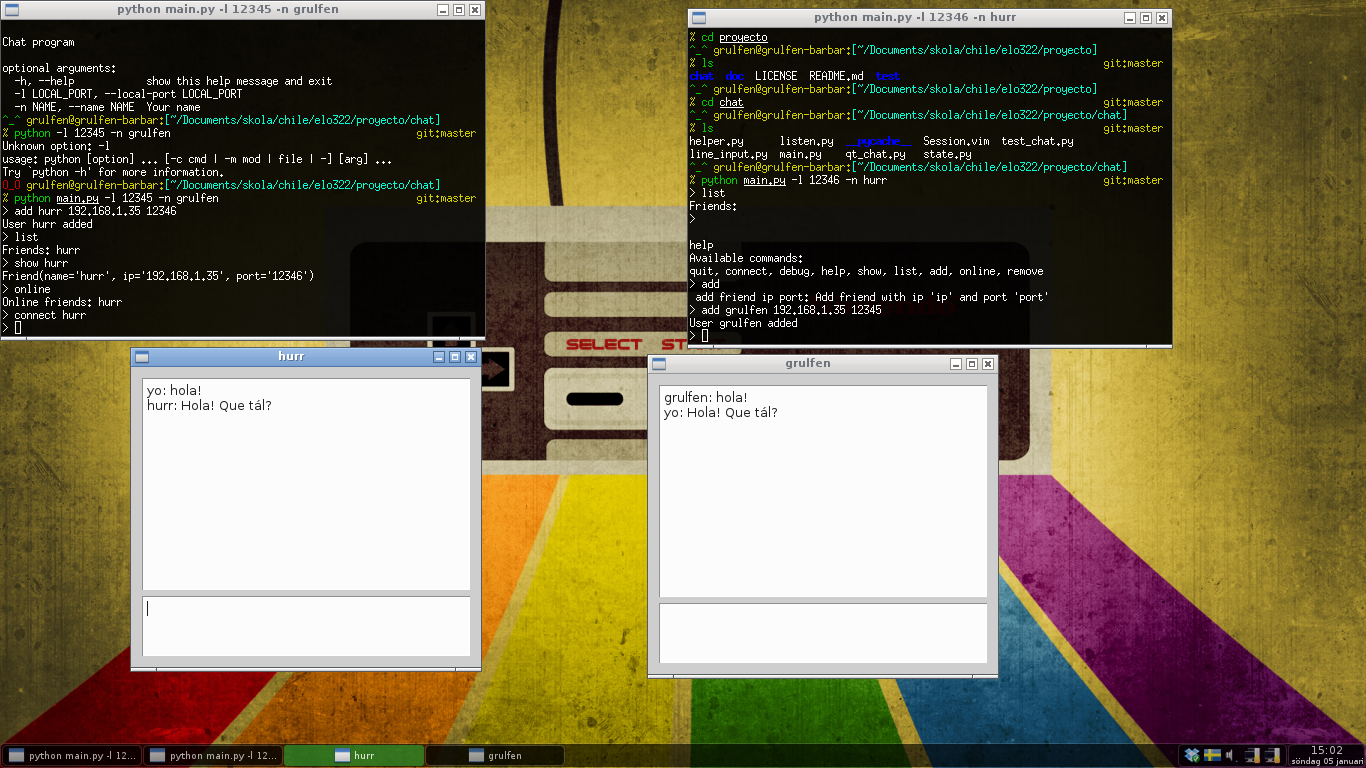
\includegraphics[width=1.2\textwidth]{../imagenes/screenshot.png}
        \caption{Screenshot de la aplicación}
        \label{fig:screen}
\end{figure}

\newpage

\section{Verificación}
Para verificar que el programa funciona bien hay el archivo
\texttt{test\_chat.py} que usa la libreria py.test. Para correr los tests
se ejecuta \texttt{py.test} en la carpeta donde está el archivo \texttt{test\_chat.py}.
Los tests se puede ver en tabla~\ref{tab:test}.
\begin{table}[h]
        \centering
        \begin{tabular}{|p{5cm}|p{8cm}|}
                \hline
                \textbf{Test} & \textbf{Descripción} \\
                \hline
                \texttt{test\_parse\_type} & Verifica el analizo del parte tipo de una mensaje \\
                \hline
                \texttt{test\_parse\_sender} & Verifica el analizo del parte enviador de una mensaje \\
                \hline
                \texttt{test\_parse\_reciever} & Verifica el analizo del parte receptor de una mensaje \\
                \hline
                \texttt{test\_parse\_body} & Verifica el analizo del parte cuerpo de una mensaje \\
                \hline
                \texttt{test\_parse\_mismatch} & Verifica el analizo cuando una mensaje está mal formateado \\
                \hline
                \texttt{test\_ping\_pong} & Verifica que se recibe un ping después de un pong \\
                \hline
                \texttt{test\_get\_msg\_hi} & Verifica que se recibe una mensaje con cuerpo hi \\
                \hline
        \end{tabular}
        \caption{Tests para verificar el funcionamiento}
        \label{tab:test}
\end{table}

\section{Uso}
Se inicia el programa con el comando \\
\texttt{python3 main.py -l PUERTO\_LOCAL -n NOMBRE}
Una linea de comandos aparece, para ver los comandos que hay se entra ``help''.
Los comandos que hay se puede encontrar en tabla~\ref{tab:comandos}. Para
recibir más información sobre un comando se entra ``help COMANDO'.

\begin{table}[h]
        \centering
        \begin{tabular}{|p{5cm}|p{8cm}|}
                \hline
                \textbf{Comando} & \textbf{Descripción} \\
                \hline
                online & Muestra los amigos que estan online \\
                \hline
                list & Muestra todos los amigos \\
                \hline
                help & Muestra ayuda sobre los comandos \\
                \hline
                add & Agrega un amigo \\
                \hline 
                debug & Muestra información para debuging \\
                \hline
                quit & Cierra la aplicación \\
                \hline
                remove & Quita un amigo \\
                \hline
                show & Muestra información sobre un amigo \\
                \hline
                connect & Abre una ventana chat con un amigo \\
                \hline
        \end{tabular}
        \caption{Comandos}
        \label{tab:comandos}
\end{table}
\end{document}
